\documentclass{article}

\usepackage{amsmath}
\usepackage{graphicx}
\usepackage{titlesec}
\usepackage{lipsum}
\usepackage{url}
\usepackage{float}
\usepackage{fullpage}
\setkeys{Gin}{width=0.50\textwidth}

\titleformat{\section}
  {\normalfont\scshape}{\thesection}{1em}{}

\title{Report 3}
\author{Vanessa Machuca and Luis Espino}

\usepackage{Sweave}
\begin{document}
\Sconcordance{concordance:Report_4.tex:Report_4.Rnw:%
1 17 1 1 0 4 1 1 18 1 9 18 1 1 7 4 0 1 2 2 1 1 5 4 0 1 2 4 1 1 2 1 0 1 %
1 31 0 1 2 1 1 1 2 1 0 4 1 3 0 1 2 3 1 1 5 1 1 1 9 3 0 1 1 2 0 1 1 2 0 %
2 2 2 1 1 16 1 2 1 16 1 2 2 1 1 15 1 2 1 15 1 2 25 1 1 6 1 2 1 1 1 13 4 %
0 1 2 13 1 1 4 12 1}

\maketitle




\section{Introduction} 

The data we are working with looks at student achievement in Portuguese course at two secondary education Portuguese schools. We found the data through the UCI Machine Learning Repository. The observational units for the dataset are students. The dataset includes demographic variables like student’s school name (binary), sex (binary), age (numeric), and whether the student lives in an urban or rural area. 

It also includes variables that relate to family, including family size, parents cohabitation status (living apart or together), mother and father's education (ordinal), mother and father’s job ('teacher', 'health' care related, civil 'services' (e.g. administrative or police), 'at$\_$home' or 'other'), student’s guardian (mother, father or other), and quality of family relations ($1$ being very bad to $5$ being excellent). 

School-related variables include home to school travel time (ordinal), weekly study time (ordinal), and number of past class failures (1-3 if $n<3$, 4 otherwise). For each of two courses, students were given a graded after the first and second period as well as a final grade.  
Academic routine, habits and performance were also measured. These variables included travel time from home to school (nominal), weekly study time (nominal), number of past class failures (nominal), reason to choose school (categorical), and number of absences (numeric). Additionally, educational resources were assessed through binary measurements of extra educational support, family educational support, extra paid classes within the course subject, extracurricular activities, attended nursery school, college aspiration, and home internet access.

Finally, nominal variables that measured more personal aspect of life included frequency of outings with friends, workday alcohol consumption, weekend alcohol consumption, current health status, and being in a romantic relationship (binary). 


\section{Task 1 - Sparse and Smooth Linear Models}

We will now run ridge regression (RR) and LASSO on the full varaible set, using cross validation to find lambda, and compare them. First up, we carry out RR, and use cross validation to determine the lambda that minimizes SSE. We omit categorical variables, as RR does not seem to like them very much. 

\begin{Schunk}
\begin{Soutput}
[1] 0.0225702
\end{Soutput}
\end{Schunk}

The lambda value which yields the lowest SSE is $0.0225702$. Now we carry out LASSO, again using CV to determine the best lambda value. 

\begin{Schunk}
\begin{Soutput}
[1] 0.03125716
\end{Soutput}
\end{Schunk}

The lambda value which yields the lowest SSE is $0.03125716$. Finally, we carry out multiple linear regression, and then use a pairs plot to compare the coefficients of all three.




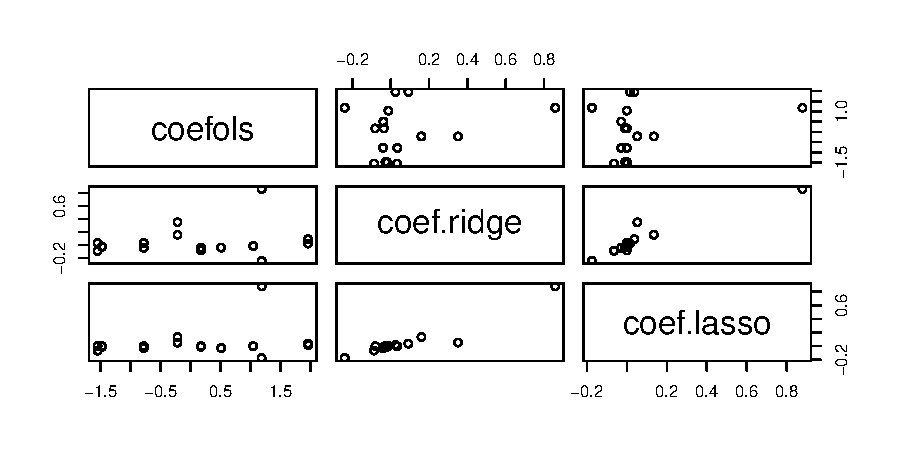
\includegraphics{Report_4-006}

The pairs plot shows that the linear model coefficients do not have high correlation with either the ridge regression or lasso coefficients. Most nonzero constants for MLR are very close to zero for ridge regression, and the biggest ridge regression coefficients are not the biggest MLR coefficients. The coefficient plot between lasso and MLR is fairly similar to the coefficient plot between ridge regression and MLR, except the coefficients hug tighter around the line x=0. Between ridge regression and lasso, most of the coefficients that hug around 0 (on both sides of 0) for ridge are positive and even closer to 0 for lasso. For both plots, only three coefficients seem to be visibly larger relative to all the other ones.


Below is a plot comparing responses predicted using MLR, RR, and LASSO. 

\bigskip
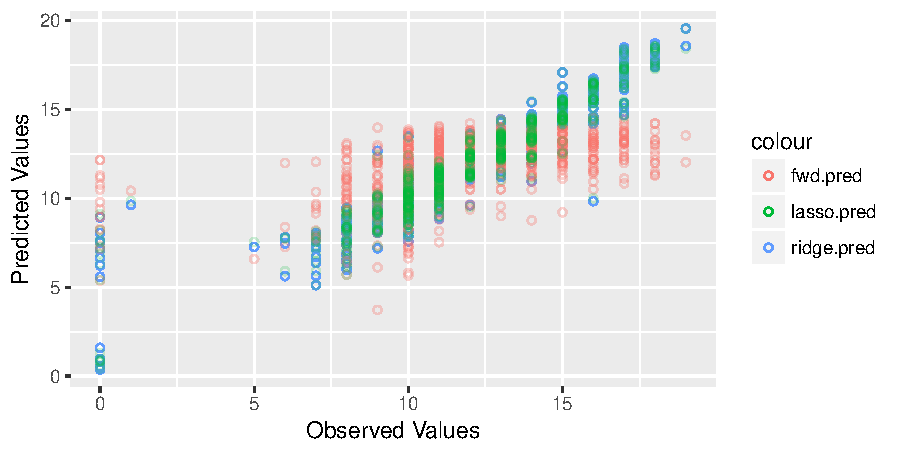
\includegraphics{Report_4-008}

Now to choose one variable and run smoothing spline and kernel smoother models on it. We change the parameters so that we have four different models for each method. We chose "absences", as this was found to be the most significant variable in report 1.  Let us first use regression splines for four different degrees of freedom: 3,4,5, and 6

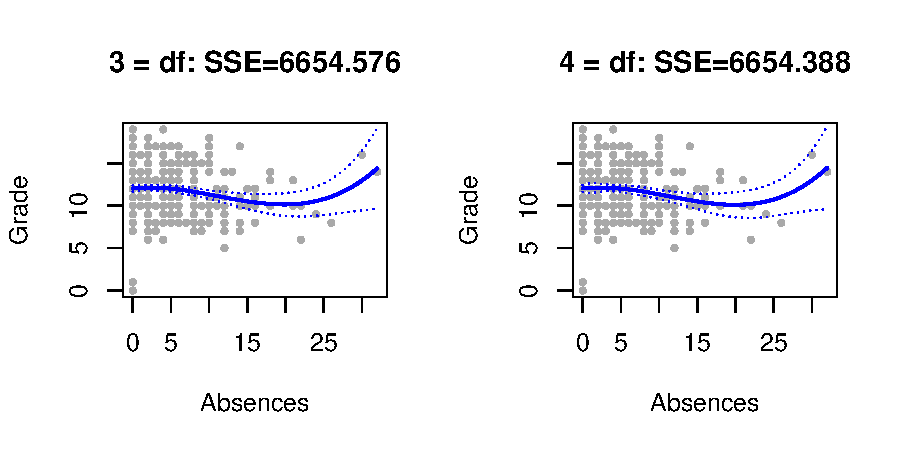
\includegraphics{Report_4-009}

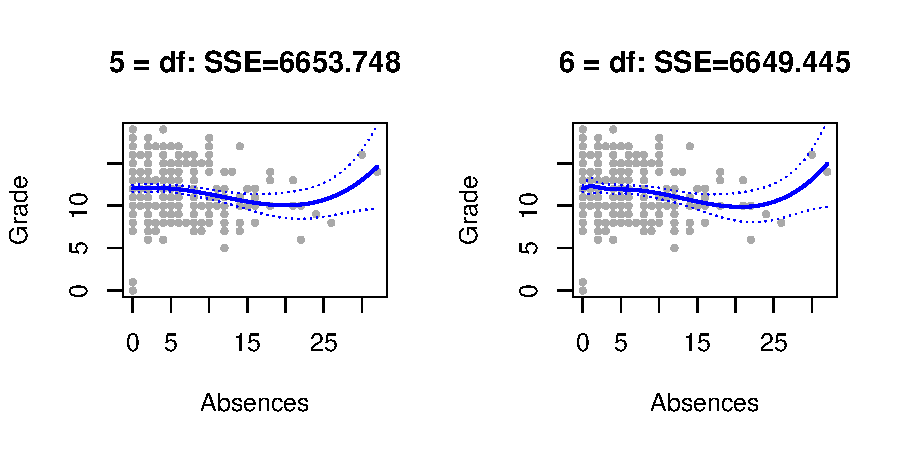
\includegraphics{Report_4-010}

6 degress of freedom minimizes the SSE. And now onward to LOESS, using span values of .6,.75,1, and 2.

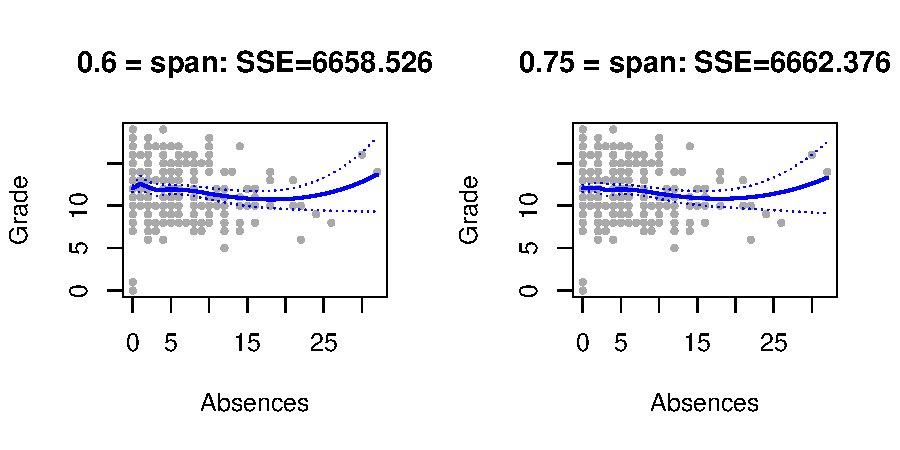
\includegraphics{Report_4-011}

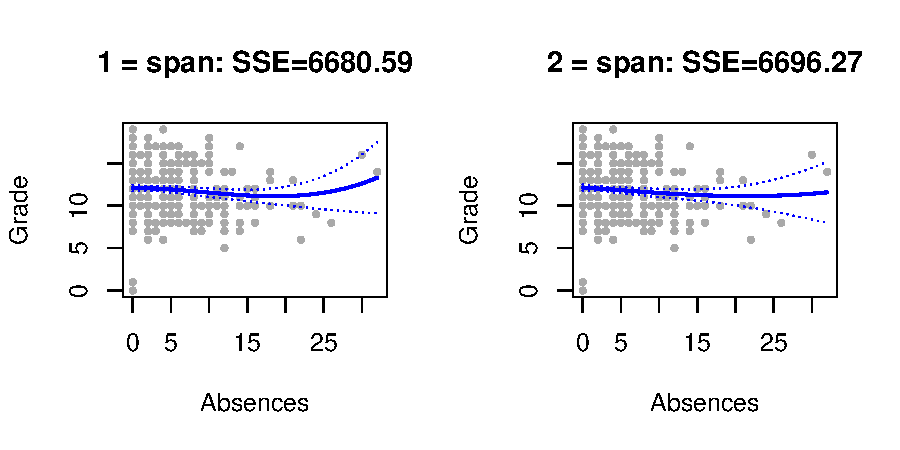
\includegraphics{Report_4-012}

A span of .6 minimizes the SSE.

Of the 8 models we generated above, then, the splines model with 6 degrees of freedom and LOESS model with span .6 minimizes the SSE, and the former begot the lowest SSE of overall. It also seems to be slightly smoother than the LOESS model. We would, then, go with the splines model.

What interested us most was how similar the models all were - at least visually. The MLR, RR, and LASSO predictions greatly overlapped with each other, as seen in the multi-color graph generated further up. And the LOESS and splines models also, upon inspection, seem almost identical. 

\section{Task 2 - Something New}

\subsection{Principal Components Regression}

Next, we perform pricipal components regression on our data. Principal components regression is a dimension-reduction technique for regression. Instead of regressing on $p$ predictors, we regress on $M$ principal components, where principal components are linear combinations of the predictors, and ideally $M<<p$. The first part of PCR is principle component analysis, where, through an iterative process, the principle components are found. This process is as follows: 

\begin{enumerate}
\item Principal component 1 is computed by finding the direction in which the observations vary the most. This is equivalent to finding the line whose distance is shortest to all the observations. 
\item Principal component 2 is computed by finding the line that is orthogonal to principal component 1 and that points in the direction in which the observations on this orthogonal plane now vary the most. 
\item Iterate as in step (2) until you've found $p$ principal components. 
\end{enumerate}

The second part of PCR is to perform a linear regression on the principal components that capture most of your variability. OLS obtains estimates for $\beta_j$ in $$y_i = \beta_0 + \sum \beta_jx_{ij} + \epsilon_i$$ that minimize $$SSE = \sum_{i=1}^{n}\left(Y_i - b_0 - \sum_{j=1}^{p-1}b_jX_{ij}\right)^2$$. On the other hand, PCR obtains estimates for $\beta_j^\prime$ in $$y_i = \beta_0^\prime + \sum_{j=1}^{p\prime}\beta_j^\prime \alpha_{ij} + \epsilon_i$$ that minimize $$SSE = \sum_{i=1}^{n}\left(Y_i - b_0^\prime - \sum_{j=1}^{M-1}b_j^\prime \alpha_{ij}\right)^2 .$$

The number of principal components is typically chosen through CV and standardizing the predictors before doing PCA ensures that all predictors have equal weight in obtaining the principal components. Otherwise, predictors with higher variance will have a greater impact on the final model.

The idea is that through $M$ principal components, where ideally $M<<p$, you can capture most of the variability in the data and the relationship with the response in less dimensions than you would through your $p$ predictors. In this way, PCR also may help prevent overfitting. A key underlying assumption of PCR is that the directions in which the $p$ predictors show the most variation are the directions associated with $Y$. 

PCR is particularly useful for data in which the response can be accurately modeled using only few principal components. We chose PCR because, based on our previous models, it seems that most of the variation in our data could potentially be captured in a few components and thus, PCR could give us a more parsimonious model compared to OLS. We also chose it because it could help address any multicolinearity present in our data.

PCR solves issues of multicolinearity, and dimensionality, where the number of observations is less than the number of predictors. 

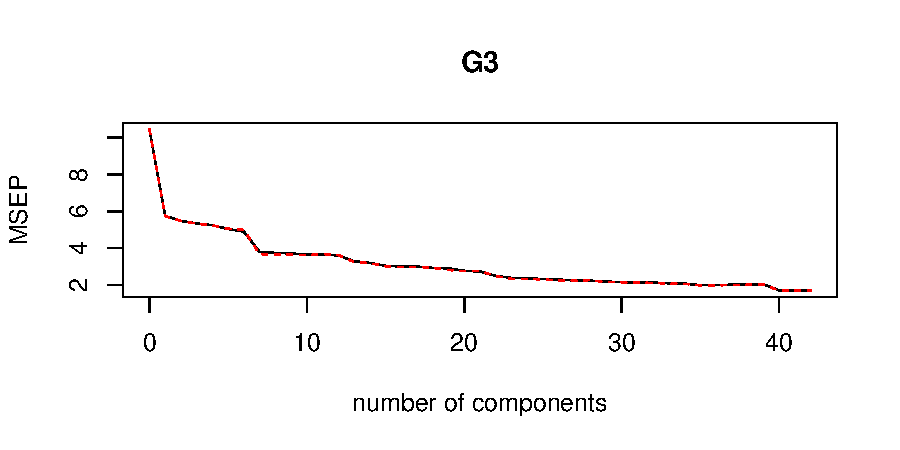
\includegraphics{Report_4-013}


\begin{Schunk}
\begin{Soutput}
[1] 7.878287
\end{Soutput}
\end{Schunk}


We chose to have 7 principal components in our model based on the CV error. The test error for this number of principal components is 6.92.

\subsection{Inverse Predictions}

So far, we have used regression models of Y on X to determine Y values from X observations. These models, though, can also be used to make inverse predictions of X on Y. That is, we might want to predict what X value led to the observed Y value. In the context of our data set, we were interested in making inverse predictions of the variable $studytime\_num$ - weekly hours studied - based on a student's grades. This might be useful for recommending study time to achieve certain grades. Obtaining inverse predictions is a matter of a simple reformulation of our usual estimated regression model

$$\hat{Y}=b_{0} + b_{1}X$$

to get 

$$\hat{X}_{h(new)} = \frac{Y_{h(new)}-b_{0}}{b_{1}}$$


Let use start, then, by generating a model of $G3$ based on $studytime\_num$. This gives us the following model

$$\hat{Y}=10.92+0.264X$$

and so 

$$\hat{X}=3.787-41.34Y.$$

Now we use the function $inverse.predict$ to make our inverse predictions:

\begin{Schunk}
\begin{Soutput}
$Prediction
[1] 15.4565

$`Standard Error`
[1] 5.148889

$Confidence
[1] 22.15388

$`Confidence Limits`
[1] -6.697379 37.610386
\end{Soutput}
\end{Schunk}

The predicted study time per week for a student with a grade of 15 is 15.46 hours per week, with a 95\% confidence interval of (-6.697,37.61). That doesn't make sense. Perhaps the data is too sparse. Let's take a look at the data.

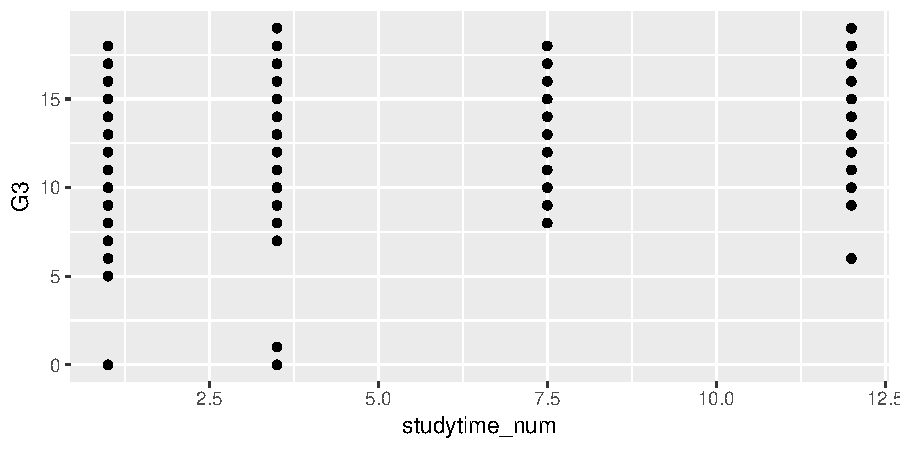
\includegraphics{Report_4-017}

Indeed, this seems to be the case.


\subsection{Tests of Assumptions}


We begin by testing whether or not there is high correlation among the continuous variables in our MLR model.

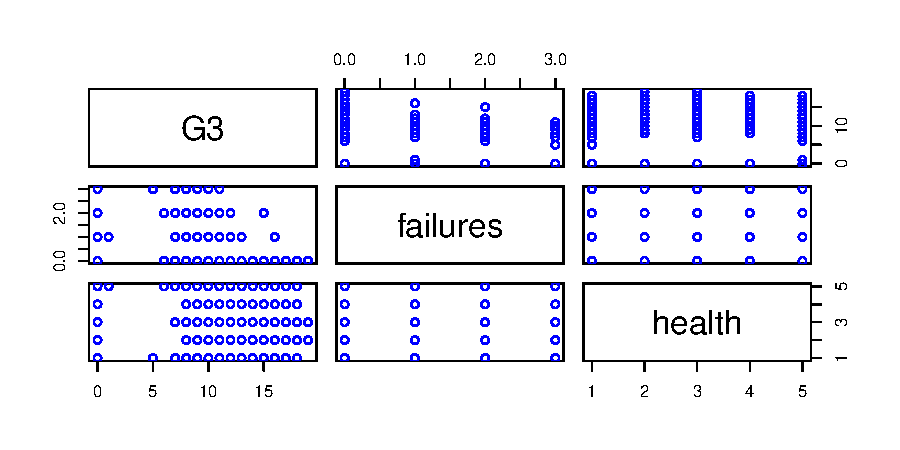
\includegraphics{Report_4-018}

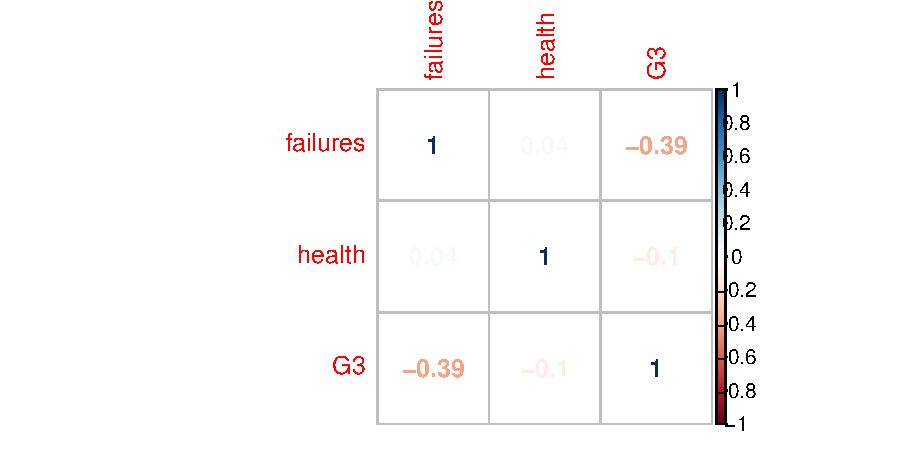
\includegraphics{Report_4-019}

Based on the correlation plots, there is moderate evidence that number of previous class failures is associated with final grade. However, there is no evidence of high correlation among the continous predictors in our MLR model. 

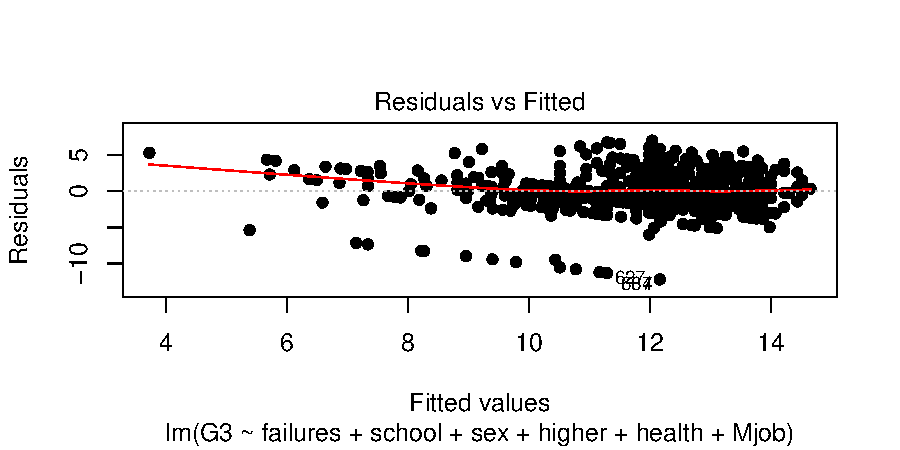
\includegraphics{Report_4-020}
\bigskip

Through a residual v. fitted plot, we notice that the residuals have unequal variance and a nonlinear shape. Thus, we apply transformations to so that the model does hold under the assumptions of equal variance and linearity. 

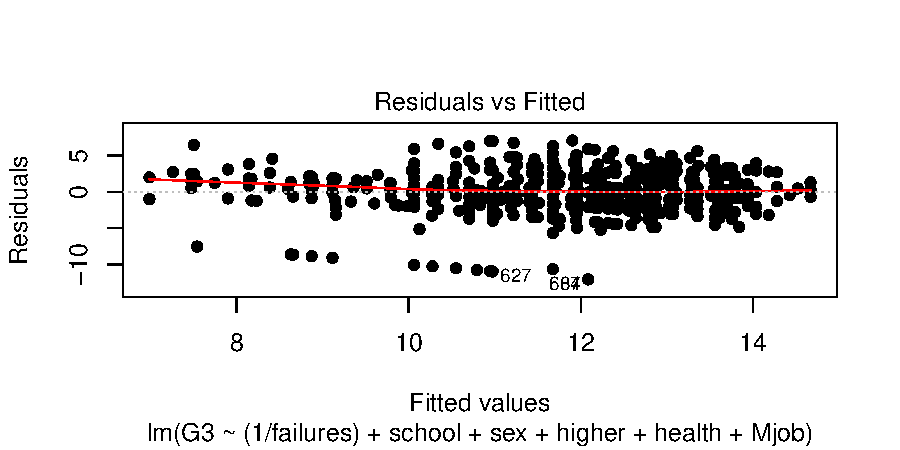
\includegraphics{Report_4-021}
\bigskip

Transforming $failures$ to $\frac{1}{failures}$ addresses both issues, though not completely. While there is improvement, a bit of nonlinearity and nonconstant variance remains. 


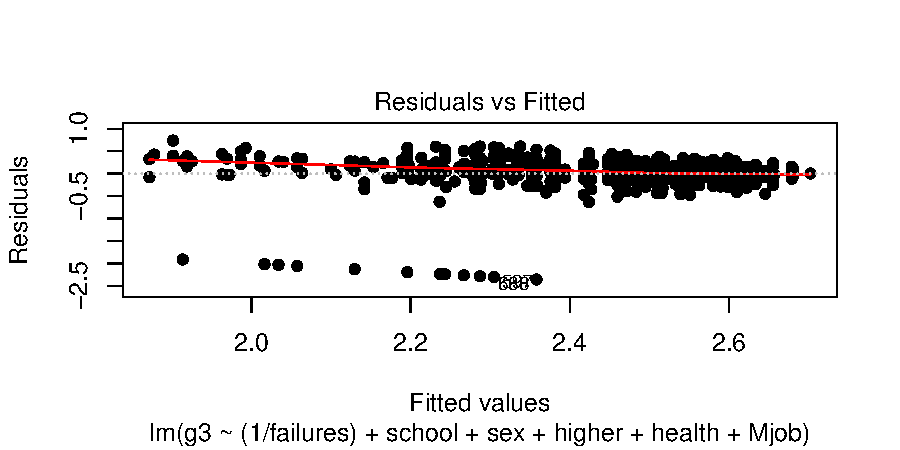
\includegraphics{Report_4-022}
\bigskip

While a Y transformation should fix the nonlinearity condition, a set of outliers with high residuals remains, which prevents us from improving the residual plot further.

Thus we keep the model with a single X transformation as our final MLR model.

\section{Task 3 - Summary}

\indent Most of the variables included in this dataset were ordinal, which prevented the analysis from being able to be more precise. The ordinal nature of many of the variables led to a very sparse dataset overall. In redoing this analysis, we would have preferred to either recode all ordinal variables to be continuous, as in the case of $study_time$, or to work with data that already included more continous and therefore, more precise variables.\\
\indent As for the model we'd recommend, all of them have their respective merits. Simpler models, like OLR, loess and RR, which all just used "absences", are easier to explain. Our client, then, might be more inclined to one of those. The stepwise model we developed in Report 3 indeed performed well, but some of the variables it included were counter-intuitive. Furthermore, we showed in this report that this model does not hold for the assumptions of linearity and constant variance. With a transformation, though, the model improved, however most conditions were still violated and this transformation reduced the $R^2$ from $0.35$ to $0.16$. The PCR model had quite a small SSE of 6.92 and addressed any multicolinearity present. Most of the variability in our data was captured in the 7 components of that model - making it quite parsimonious relative to the 34 predictors we could have used. 

\end{document}
